% WSCG sample document 
%
% based on Gabriel Zachmann's sample
% http://zach.in.tu-clausthal.de/latex/
%
% modified Apr 2012 to match WSCG Word template
%
\documentclass[twoside,twocolumn,10pt]{article}
%\documentclass[twoside,twocolumn,draft]{article}

%  for debugging
%\tracingall%\tracingonline=0
%\tracingparagraphs
%\tracingpages


%%%%%%%%%%%%%%%%%%%%%%%%%%%%%%%%%%%%%%%%%%%%%%%%%%%%%%%%%%%%%%%%%%%%%%%%%%%%%
%                             Packages

\usepackage{wscg}           % includes a number of other packages (e.g., myalgorithm)
\RequirePackage{ifpdf}
\ifpdf
 \RequirePackage[pdftex]{graphicx}
 \RequirePackage[pdftex]{color}
\else
 \RequirePackage[dvips,draft]{graphicx}
 \RequirePackage[dvips]{color}
\fi
%\usepackage[german,english]{babel}     % default = english
%\usepackage{mypicture}      % loads graphicx.sty, color.sty, eepic.sty
%\usepackage{array}          % better tabular's & arrays, plus math tabular's
%\usepackage{tabularx}      % for selfadjusting p-columns
%\setlength{\extrarowheight}{1ex}   % additional space between rows
%\usepackage{booktabs}      % typographically much better
%\usepackage{mdwlist}        % for compacted lists, and more versatile lists
%\usepackage[intlimits]{amsmath} % more math stuff, see texdoc amsldoc
%\usepackage{mymath}         % own commands, loads amssymb & array.sty
%\usepackage{hyphenat}      % hyphenatable -, /, etc.
%\usepackage{theorem}
%\usepackage[sort&compress]{natbib}% better \cite commands, more flexible
%\usepackage[sort&compress,super]{natbib} % better \cite commands, more flexible
%\newcommand{\citenumfont}[1]{\textit{#1}}


\usepackage{nopageno}       % no page numbers at all; uncomment for final version

\usepackage{subfig}
\usepackage{graphicx}
%%%%%%%%%%%%%%%%%%%%%%%%%%%%%%%%%%%%%%%%%%%%%%%%%%%%%%%%%%%%%%%%%%%%%%%%%%%%%
%                                Title

\title{Automatic morphology: Application on biological images}

\author{
  \hspace{-0.1\textwidth}
  \parbox{0.2\textwidth}{\centering
    LE Van \\
    Linh\\[1mm]
LaBRI-CNRS 5800\\
ITDLU, Dalat Univ-V
linhlv@dlu.edu.vn/ van-linh.le@labri.fr
}
\hspace{0.02\textwidth}
\parbox{0.2\textwidth}{\centering
BEURTON-AIMAR Marie\\[1mm]
LaBRI-CNRS 5800\\
Bordeaux University\\
33400 Talence-F\\
beurton@labri.fr
}
\hspace{0.02\textwidth}
\parbox{0.25\textwidth}{\centering
KRAHENBUHL \\Adrien\\[1mm]
LaBRI-CNRS 5800\\
Bordeaux University\\
33400 Talence-F\\
adrien.krahenbuhl@labri.fr
}
\hspace{0.02\textwidth}
\parbox{0.18\textwidth}{\centering
PARISEY\\ Nicolas\\[1mm]
IGEPP\\
INRA 1349\\
35653 Le Rheu-F\\
nparisey@rennes.inra.fr
}
}

%%%%%%%%%%%%%%%%%%%%%%%%%%%%%%%%%%%%%%%%%%%%%%%%%%%%%%%%%%%%%%%%%%%%%%%%%%%%%
%                          Hyperref


% no hyperlinks
\usepackage{url}
\urlstyle{tt}

% Donald Arsenau's fix for missing kerning of "//" and ":/"
\makeatletter
\def\Uslash{\mathbin{\mathchar`\/}\@ifnextchar{/}{\kern-.15em}{}}
\g@addto@macro\UrlSpecials{\do \/ {\Uslash}}
\def\Ucolon{\mathbin{\mathchar`:}\@ifnextchar{/}{\kern-.1em}{}}
\g@addto@macro\UrlSpecials{\do : {\Ucolon}}
\makeatother





%%%%%%%%%%%%%%%%%%%%%%%%%%%%%%%%%%%%%%%%%%%%%%%%%%%%%%%%%%%%%%%%%%%%%%%%%%%%%
%                              My Commands


%\DeclareMathOperator{\sgn}{sgn}

%\theorembodyfont{\upshape}
%\theoremstyle{break}
%\theoremheaderfont{\bfseries\normalsize}

%\newtheorem{lem}{Lemma}
%\newtheorem{defn}{Definition}



%%%%%%%%%%%%%%%%%%%%%%%%%%%%%%%%%%%%%%%%%%%%%%%%%%%%%%%%%%%%%%%%%%%%%%%%%%%%%
%                                Document


\begin{document}

\twocolumn[{\csname @twocolumnfalse\endcsname

\maketitle  % full width title


\begin{abstract}
\noindent
  Phenotype of species are characterized by several informations like,
  age, sex, morphological measures and environment parameters. Biologists are
  familar to manually getting morphological measures. In the case of
  analysis at the macro level (tissues, small parts of animal \ldots)
  that can be done directly by measuring the element geometry: length,
  width, diameter, angles \ldots. Another way is to take pictures of
  these elements and to run image processing algorithms. From a
  collection of beetle pictures, we have initiated this work to test the
  feasability of automatically positionning landmarks on biological
  images. The set of images contains 293 beetles and for all an image of the left
  and right mandibles. For each mandible, a set of 16 and 18
  landmarks (resp. left and right) have been set manually. In a previous
  work\cite{leestimating} based on Palanaswami article \cite{palaniswamy2010automatic} we have shown that
  if we consider the centroid measure of the mandible as the parameter
  to obtain, the probabilistic Hough Transform can provide very
  interesting results. But in the case of the main goal is to fix
  landmarks to get property about specific area (defined by
  biologists) the result is not as precised as we have expected. In this
  next turn, we have kept the same method to segment and to register
  scene images with model but we have change the way to set the
  model landmarks on the scene. This new procedure uses a SIFT
  algorithm as the last operation of our process. We will compare all
  the obtained results in order to define the new workflow to label
  the mandible images.
\end{abstract}

\subsection*{Keywords}
Automatic morphology, landmarks identification, image registration.

\vspace*{1.0\baselineskip}
}]



%%%%%%%%%%%%%%%%%%%%%%%%%%%%%%%%%%%%%%%%%%%%%%%%%%%%%%%%%%%%%%%%%%%%%%%%%%%%%


\section{Introduction}

\copyrightspace

In biology, morphology analysis is widely used to keep the changing
information of the organism or detecting the difference information
between the organisms. From the result of morphology analysis, we can
conclude the evolution of an organism family, or we may classify the
organisms. Especially in agriculture, morphology is one of best ways
to learn about the variations of the insect on crops. The morphology
methods may be divided into the groups by the features which are used
by the methods such as shape, structure, color, pattern or size of the
object. In the aim to study the potential links between these
variations and agricultual ecosystems, a set of 291 beetles has been
collected with all the information about the sex, place where they are
found and agricultural practices in each field were recorded. For each
beetle, the morphometric landmarks has been defined on each part (each
insect includes five parts: head, pronotum, body, left and right
mandible) of the insect by the biologies. In this context, we try to
indicate the landmarks on two parts of beetle (left and right mandible
(see figure \ref{figparts})). Morphometric landmarks are points that
can be defined in all speciemns and located precisely. Landmarks are
widely used in many biological studies and they are currently included
into the classification procedures.\\[0.1cm]

\begin{figure}[h]
\centering
\subfloat[Left mandible]{\label{figrbox2}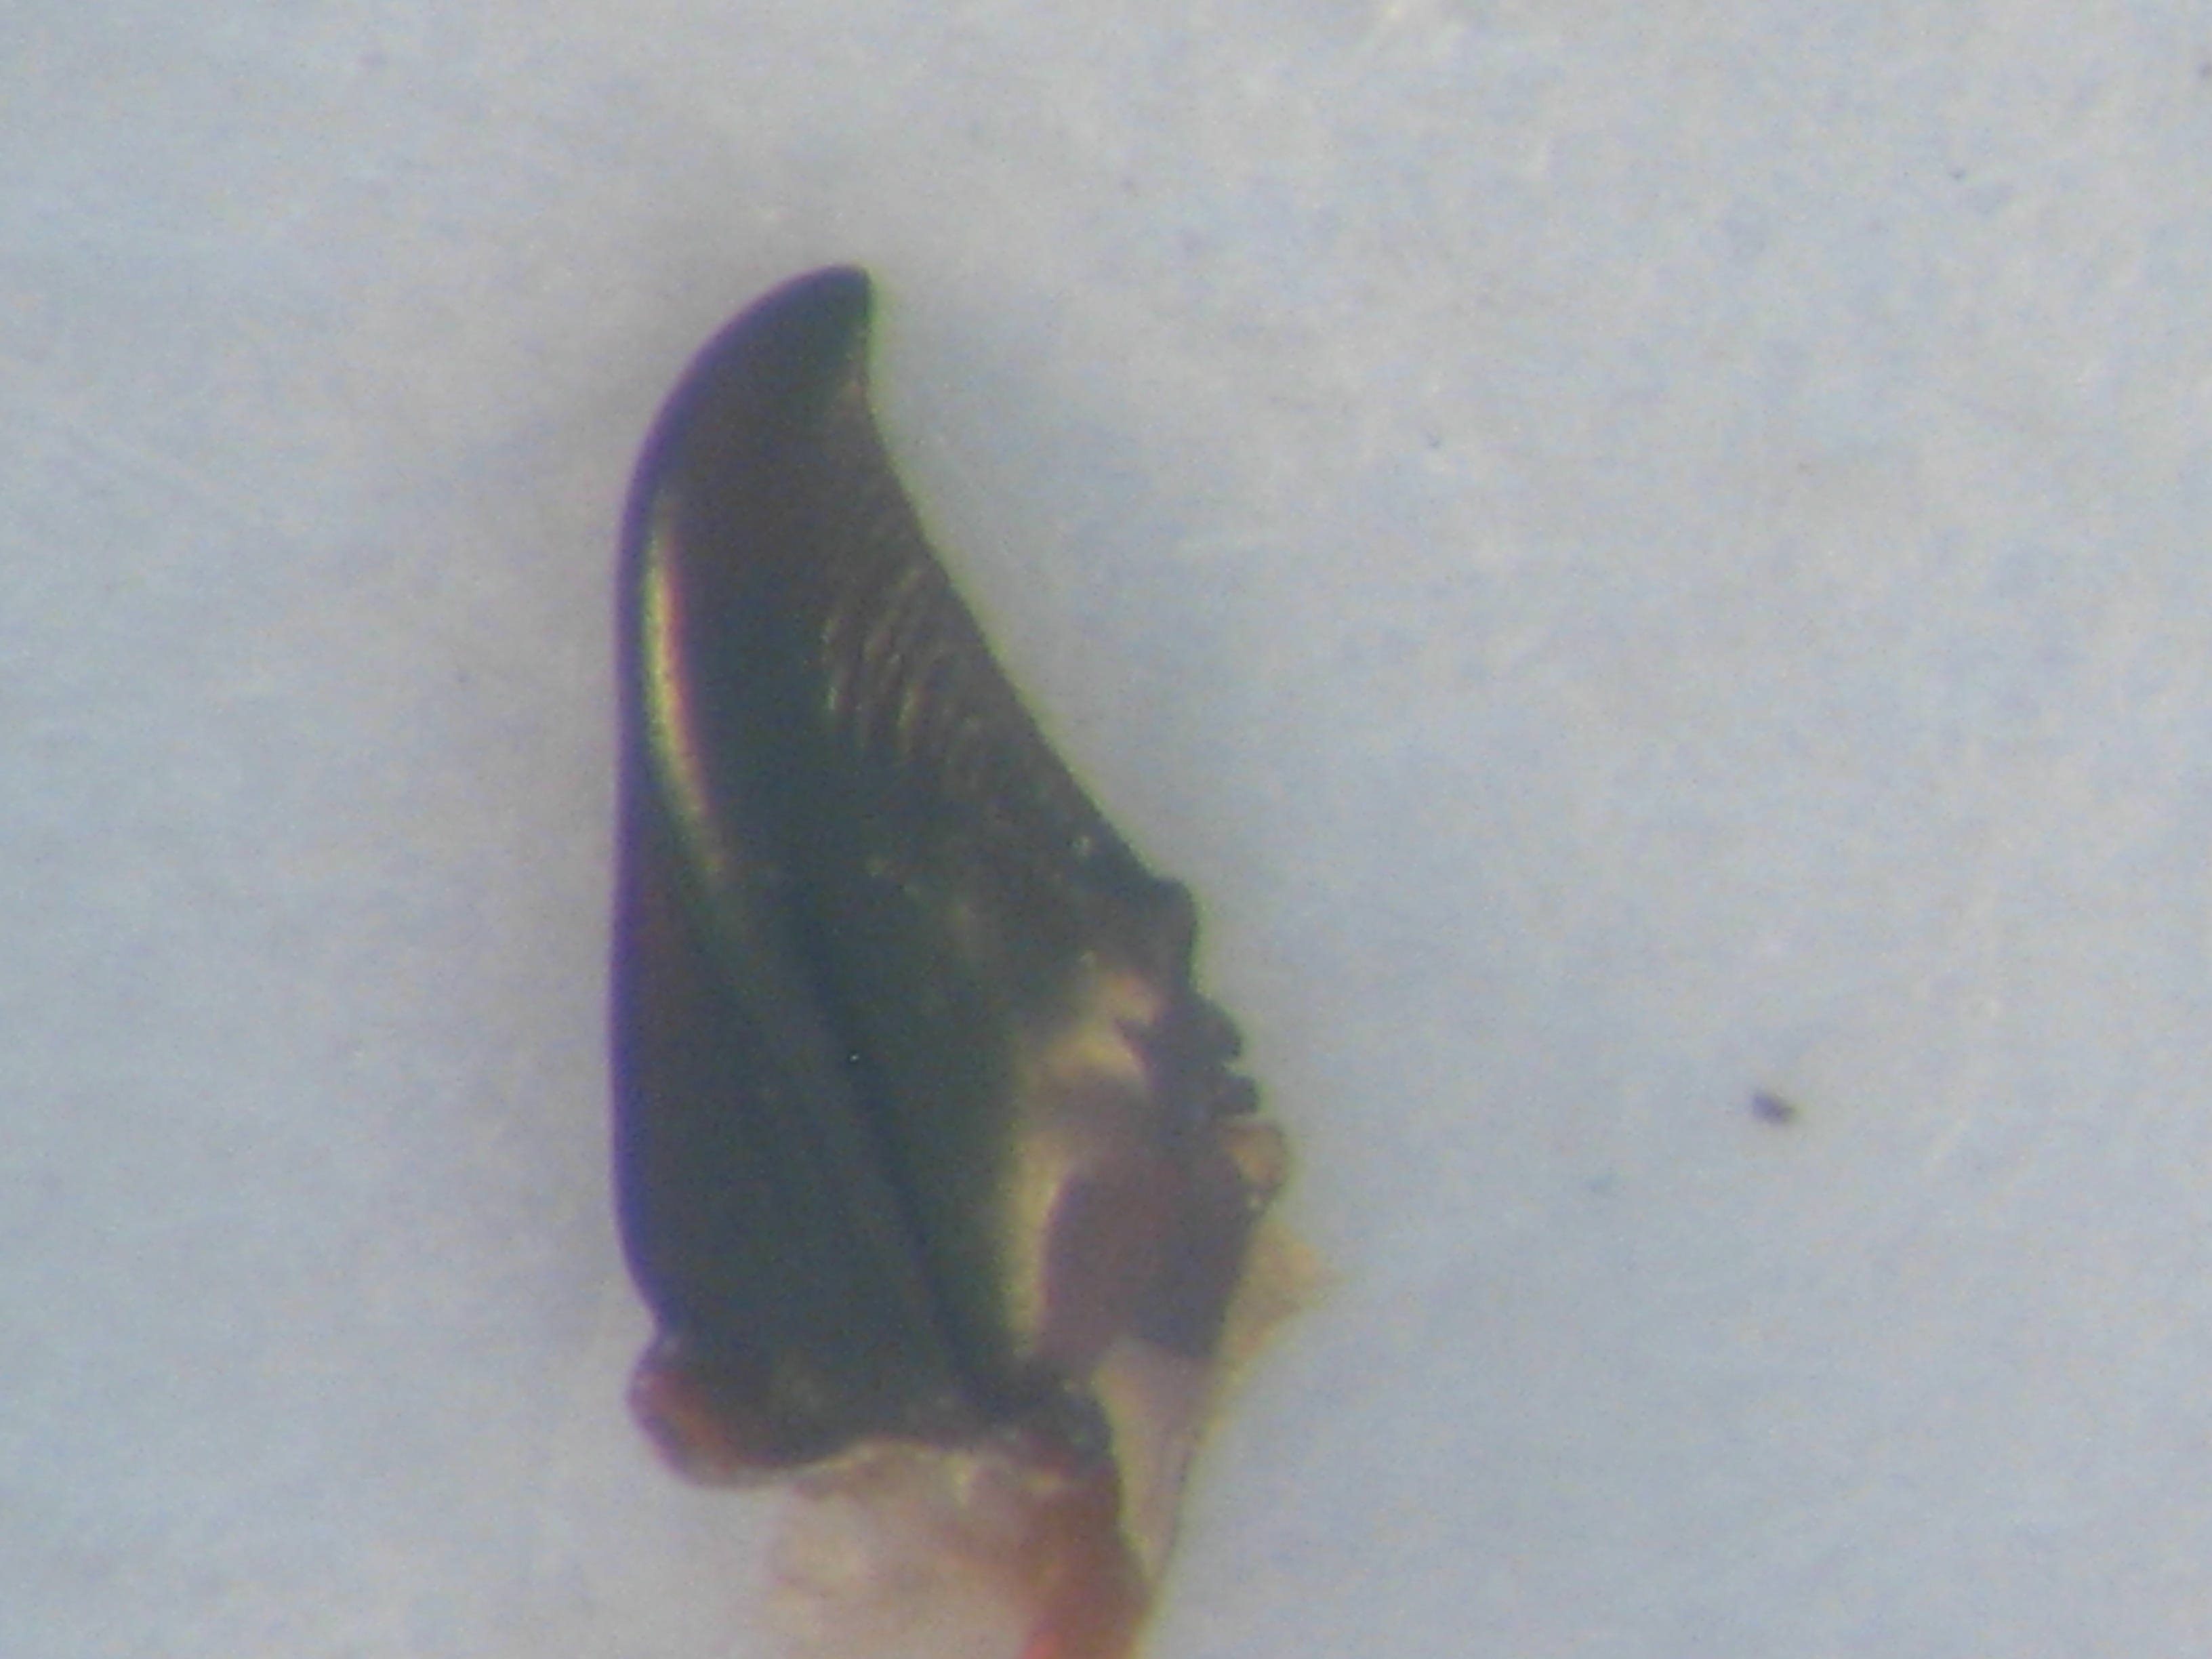
\includegraphics[width=0.22\textwidth]{./images/lm}}~~
\subfloat[Right mandible]{\label{figrbox1}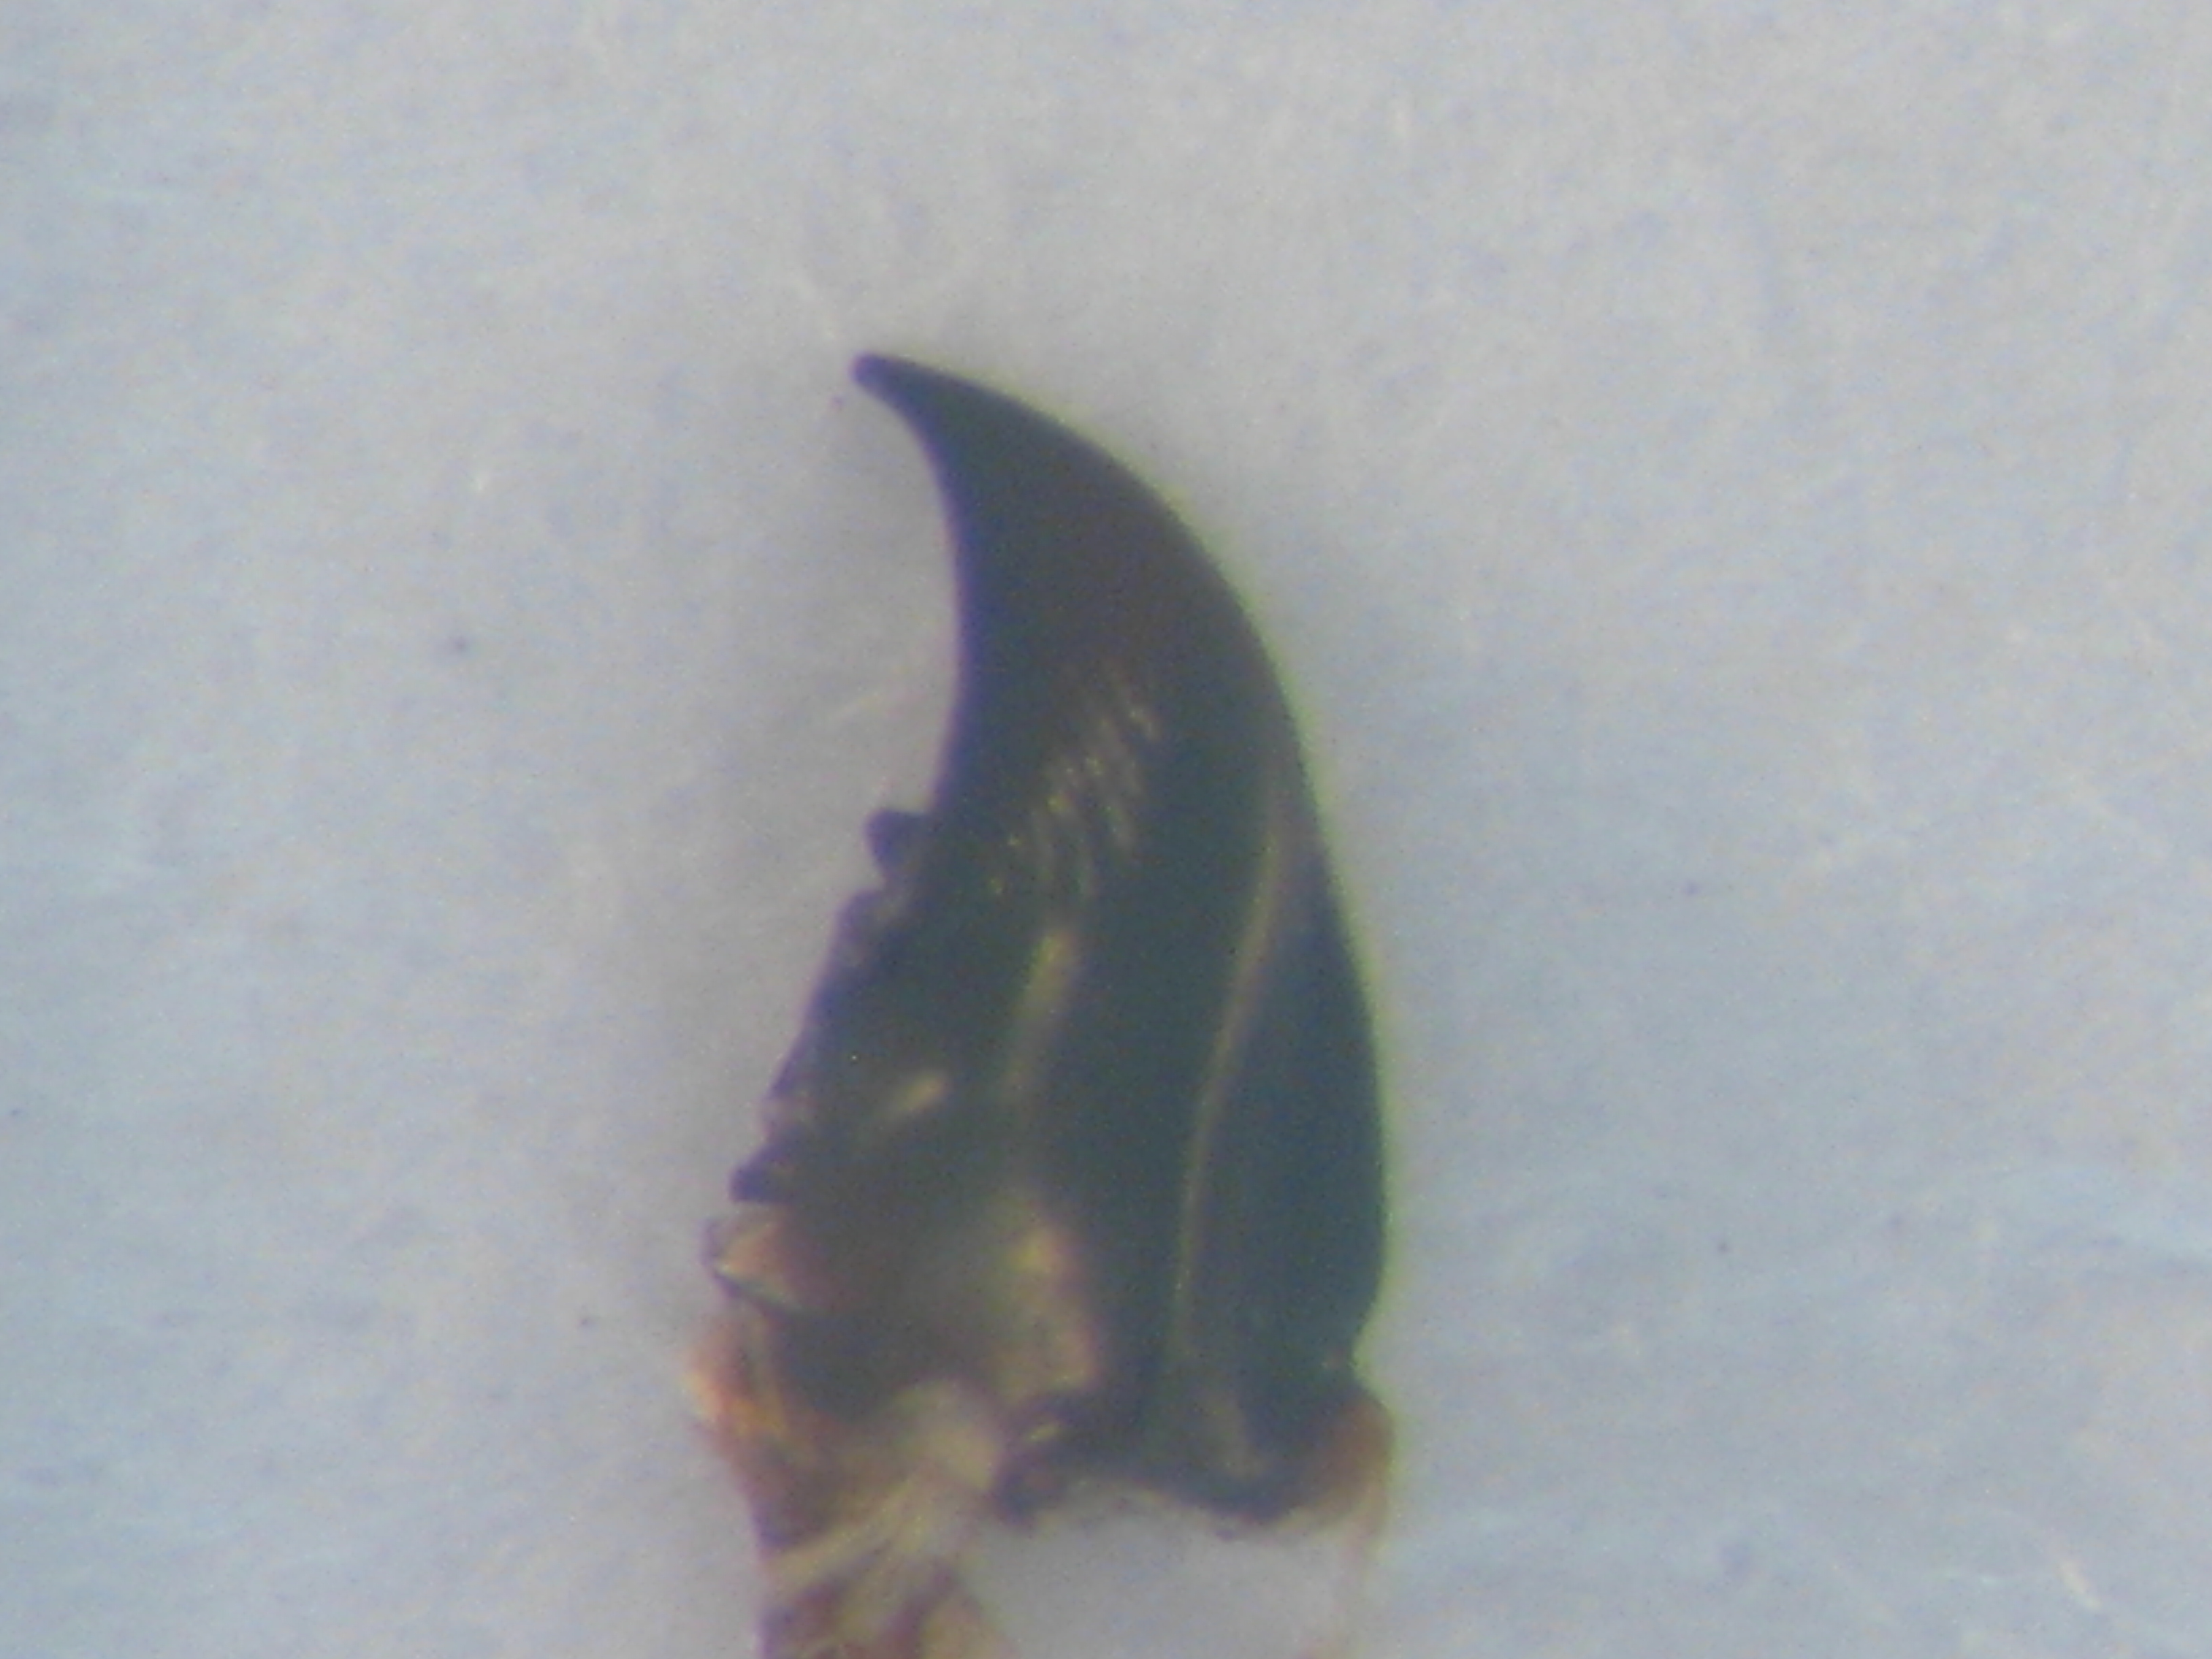
\includegraphics[width=0.22\textwidth]{./images/rm}}
\caption{The mandibles of beetle}
\label{figparts}
\end{figure}~\\[0.1cm]
In this paper, we focus on a method that can automatic identification
of landmarks on 2D images of beetle, specify the mandibles of
beetle. Through whole the article, we use two images to automatic
extraction the landmarks: model image and scene image. The method
mainly includes four stages: firstly, we extract the features of the
object in the image; secondly, generalizing Hough transform is used to
detect the presence between two images; thirdly, the translation and
rotation is identified by image registration; finally, a refinement of
the estimated landmarks is done by comparing the descriptors  between
model landmarks and estimated landmarks.\\[0.1cm]

In section 2, the steps of our methods will be discussed. All
experiments and evaluation are described in section 3. Finally, we
have some conclusion in section 4.

\section{Method}
For each image, a set of manual landmarks have been set by biologists
corresponding to the morphological points of interest (18 landmarks
for each right mandible and 16 landmarks for each left mandible). The
automatic procedure to determine the landmarks is based on the
segmentation of the image. The presence between two images are
indicated by generalizing Hough transform, along with theirs
translation and rotation are determine by applying registration. The
last step is using descriptors measure (L2 distance) to verify the
location of estimated landmarks.

\subsection{Image segmentation}
In the methods of image processing, feature extraction is always a
important stage. Besides, depending on the nature of the method, the
methods are applied before (pre-processing) or after (post-process)
extracting the features. In our method, the original Canny
alogrithm\cite{canny1986computational} is idea for detect the curves on the image. The
ratio between lower threshold and upper threshold which are used in
Canny algorithm is 1:3 (lower threshold approximated to 1 times
\textit{threshold value} and upper threshold set to 3 times threshold
value). This value is evaluated by the experiments. The
\textit{threshold value} has been determined by analyzing the image
histogram. During appling the Canny alogrithm to detect the curves of
object, the gradient direction of each pixel which belongs to the
curves is kept for the next steps of the method.

\begin{figure}[h]
\centering
\subfloat[Segmentation result after applying Canny
  algorithm]{\label{canny1}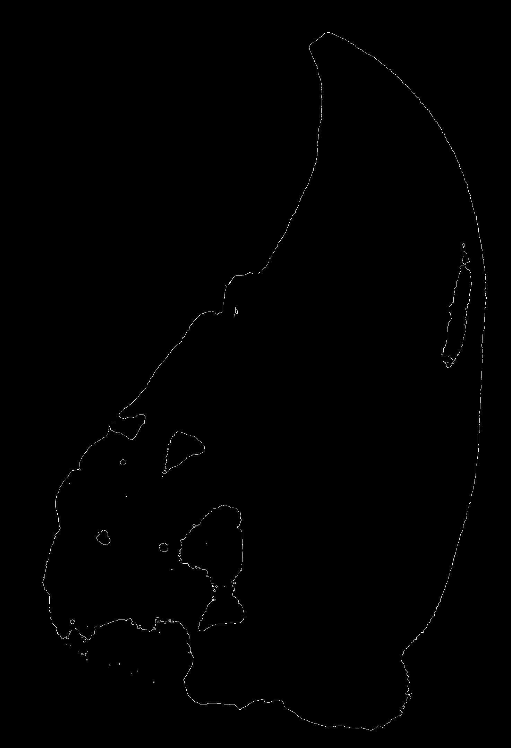
\includegraphics[width=0.2\textwidth]{./images/canny1}}~~ 
\subfloat[Segmentation result after applying Canny algorithm and
  post-process]{\label{canny2}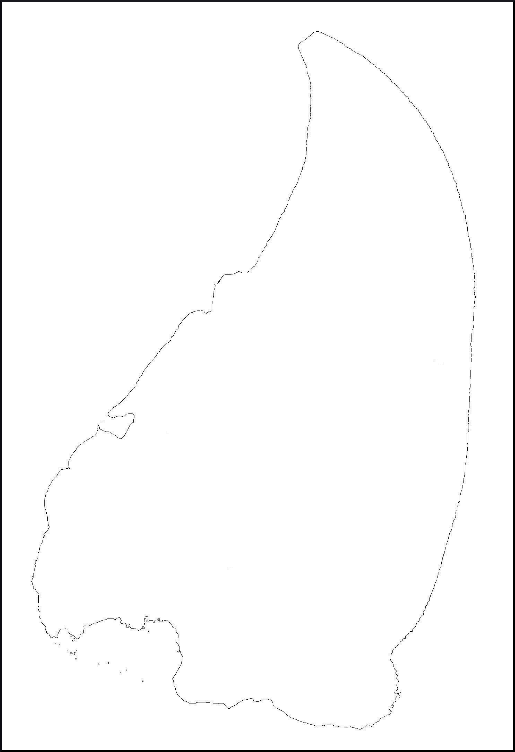
\includegraphics[width=0.2\textwidth]{./images/canny2}} 
\caption{The segmentation results of the image}
\label{canny}
\end{figure}~\\
In this study, the aim of segmentation stage is determined the outer
border of the object which can be used to reconstruct the shape of the
object as well as provide the best data for next step. The curves from
Canny algorithm will be post-processed to remove the unnecessary
curves i.e hole inside the border (see figure \ref{canny}).

\subsection{Generalizing Hough transform}
The generalizing Hought transform (GHT)\cite{ballard1981generalizing} is one of the
keys of this study. With two input images, GHT is used to recognize
the presence between two images. The GHT includes two
phases: training and recognition.\\[0.1cm]

\begin{figure}[htb]
    \centering
    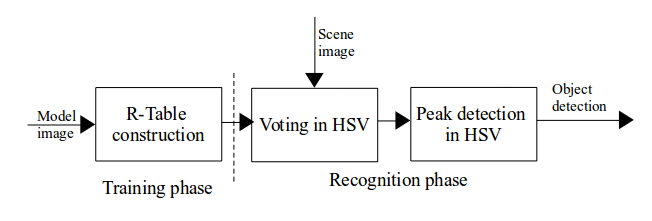
\includegraphics[width=0.5\textwidth]{./images/ghtdiagram}
    \caption{Block diagram of GHT}
    \label{fig:box}
\end{figure}~\\

In the training phase of GHT, model image is used to construct
R-table. This is table that contains the polar value of each point on
model's curves (the result of segmentation). A polar coordinate system
is initialized in the model image by fixing a reference point and
using it as origin. The R-table records the polar coordinate values of
all boundary points. The rows of R-table are indexed by the gradient
directions of the points on the curves. It means that with a gradient
direction can be exists many polar coordinate values.

\begin{table}[htb]
	\centering
	\begin{tabular}{|l|l|l|l|}
	\hline
	Index & Polar values \\
	\hline
	gradient 1 & (r1,l1), (r2,l2),(r3,l3) \\
	\hline
	gradient 2 & (r2,l2),(r4,l4),(r1,l5),... \\
	\hline
	... & ...\\
	\hline
	gradient n & (r1,l1),(r4,l5),(r5,l5),... \\
	\hline
	\end{tabular}
	\caption{An example of R-Table}
\end{table}~\\

During the recognition phase, a 2D accumulator is used, called Hough
Space Voting (HSV). The axes of HSV express for the information of
polar coordinate system. For each point on scene's curves, we try to
find a record in R-table that corresponding with the gradient
direction of each scene point. The voting will be carried out at all
location in HSV that found in R-table. At the end of voting process,
if the scene image is identical to the model image, then the cell
where have the highest number of votes corresponds to the reference
point of the model in the scene image. Besides, the peak value would
be equal to the number of curve points of the scene image when the
model and scene image match perfectly.

\subsection{Image registration}
Our study is working on the 2D image, and the transformation between
two images are inevitable. Though, GHT is just hired to detect the
presence of the model image in the scene image. Translation and
rotation are determined by applying an alignment method based on the
set of boundary points of two images. In this case, we use Principal
Component Analysis Iteration (PCAI) to finish this work. This method
is improved from PCA method\cite{shlens2014tutorial}. Firstly, the centroid point of each image is defined by getting the mean coordinate of all boundary points. Secondly, a principal axis of the images are indicated, this is a connected line from centroid point to a point in the list of curve points. For each point in the curve, we create a line from centroid point to them and assume it as an axis. The mean perpendicular distance from the remaining points to the axis are calculated. This work is finished for all points on the curve, and the principal axis is the line that has the minimum mean perpendicular distance to other points. The translation is
indicated by translation between two centroid points. The rotation is
the angle between the principal axis of two images. As well as, the
rotation direction is determined by checking each direction. However,
in some case, the translation and rotation between two images are
wrong indicated. To make sure that we have obtained the best match
between the images. We applied an iteration to get the best register
of them. And instead consider all the points in the curve, we just
need to consider a subset of it. For that, the curve points are sorted by
y-coordinate first. Then a half points are extracted to check. The
PCAI is applied on two new subsets until obtaining best matching of
two images. Figure \ref{fig:box} shows two curves after registration by PCAI. 
The aquamarine curve and blue curve are segmentation of the model and the scene image, respectively.
At the end of PCAI, a hypothesis is made to judge the scale between the images. For each image, the bounding boxes are indicated by the coordinates of the points on the curve. The scale of x and y-direction are determined by the ratio between the corresponding sides of the bounding boxes. Then, the scene curve is scaled to fit the model curve.
\begin{figure}[htb]
    \centering
    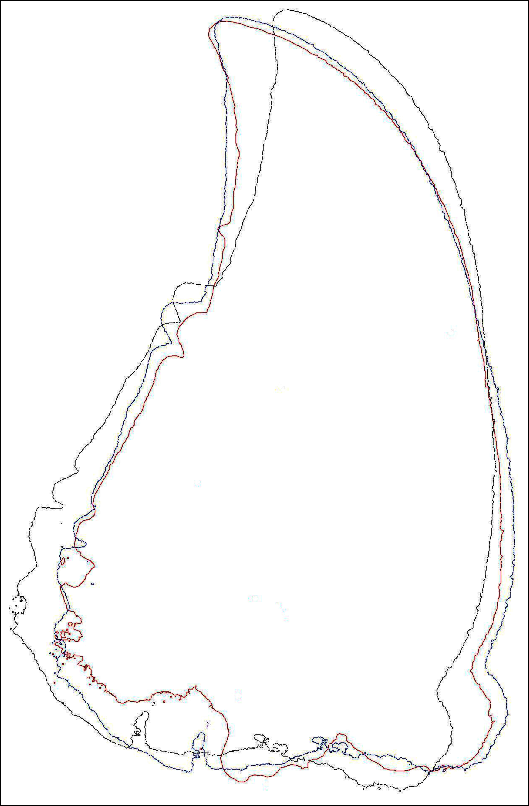
\includegraphics[width=0.2\textwidth]{./images/imreg}
    \caption{A registration result between two images.}
    \label{fig:box}
\end{figure}~\\

At the result of PCAI, we have the fitting between model and scene. The landmarks of the scene
image are estimated by the manual landmarks of model image. Hence, before estimating the
landmarks, a translation and rotation are applied on scene image to
match the pose between the scene and the model. 

\subsection{Refinement the estimated landmarks}
The GHT and registration step gave us the estimated coordinate of
scene's landmarks. But sometimes the landmarks can stay at the
incorrect location. For this reason, at the end of the method, we
apply descriptors measure\cite{lowe2004distinctive} to verify the location of
estimated landmarks. The location of manual and estimated landmarks
are presented as the descriptors. Then, the L2 distance is applied to
measure the distance between them. The equation of L2-distance is
given by equation (\ref{eq:cross-correlation}).

\begin{equation}
\label{eq:cross-correlation}
	L(x,y) = \sum\limits_{x_i,y_i}\sqrt{(x_i-y_i)^2}
\end{equation}
Where $x_i, y_i $ are the corresponding location in the descriptors.\\[0.2cm]
For each manual landmark in the model, a sub-image \textit{$I$} with
the size \textit{$s_1$} is created; and the corresponding estimated
landmark on the scene, a template \textit{$T$} with the size
\textit{$s_2$} is created (\textit{$s_1 < s_2$}). For each pixel in
\textit{$I$}, the orientation and gradient magnitude are
calculated. The descriptor is created for image \textit{$I$}. This is
a histogram with 8-bins of orientation and the length of each bin in the histogram is the sum of
the gradient magnitude of corresponding orientation. For each pixel in template \textit{$T$}, a
sub-template \textit{$T^{'}$} is extracted with the same size of
image \textit{$I$} and its descriptor is calculated with the same way
with image \textit{$I$}. Then the distance between image \textit{$I$}
and sub-template \textit{$T^{'}$} is calculated. The last location of
estimated landmarks is the pixel in template \textit{$T$} that has the smallest measure
distance value. Finally, the automatic landmarks are inverted to match
with the real location in the scene image (by inverting the
transformation and rotation).
\begin{figure}[h]
\centering
\subfloat[Result on right mandible]{\label{figrsmd}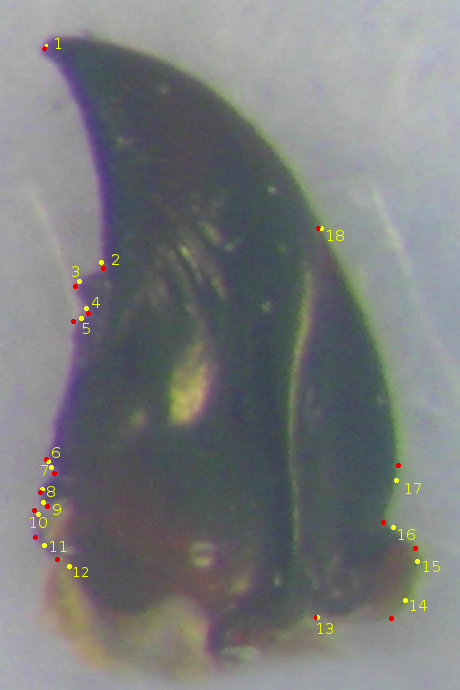
\includegraphics[width=0.22\textwidth]{./images/md_rs}}~~
\subfloat[Result on left mandible]{\label{figrsmg}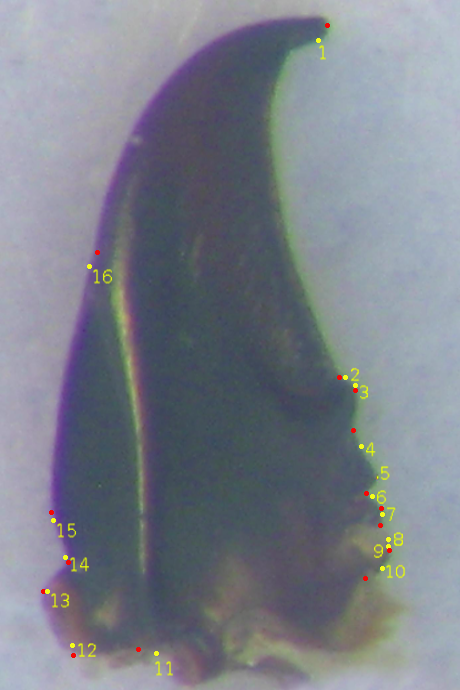
\includegraphics[width=0.22\textwidth]{./images/mg_rs}}
\caption{The automatic landmarks on mandibles}
\label{figresult}
\end{figure}~\\
Figure \ref{figresult} shows a complete result on one scene mandible with the manual landmarks (red points) and estimated landmarks (yellow points).
\section{Experiments and result}
All the steps in our method are implemented in MAELab\footnote{MAELab
  is a free software in C++. It can be directly obtained by request
  the authors.}. Two sets of beetle have been analyzed, right and left
mandible. After verifying the quality of the image, it remains 288
usable images for right mandible and 285 images for left mandible. The
removed images include the images that do not contain the mandible and
the mandible is broken.\\

In all valid images, a set of 18 manual landmarks of right mandible
(16 landmarks for left mandible) are indicated by biologists. Along
with choosing the centroid size to measure the mandible. This size is
obtained by sum of all square distance from each landmarks to the
centroid point (see \cite{web2010}).

\begin{figure}[htb]
    \centering
    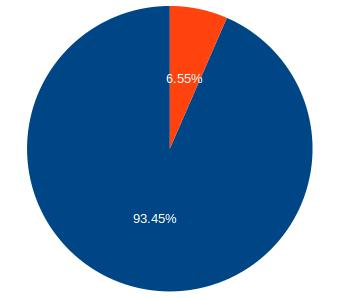
\includegraphics[width=0.3\textwidth]{./images/mdresult}
    \caption{The percentage of correct proportions on right mandibles }
    \label{figmdresult}
\end{figure}~\\
\begin{figure}[htb]
    \centering
    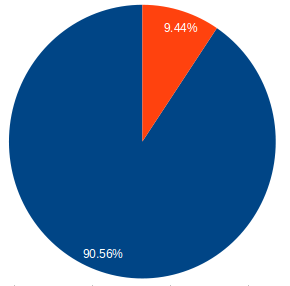
\includegraphics[width=0.3\textwidth]{./images/mgresult}
    \caption{The percentage of correct proportions on left mandibles }
    \label{figmgresult}
\end{figure}~\\
By this way, we have compared the centroid size between manual
landmarks and estimated landmarks. We can see in figure
\ref{figmdresult} and figure \ref{figmgresult} for all images. The
correct proportions of estimated landmarks are 94,48\% for the right
mandible and 90,56\% for the left mandible. The experiment is done by choosing an arbitrary 
image in the dataset as the model. The automatic landmarks are estimated on remaining images with the method that we have described. Then, the centroid size of each image is calculated and evaluated. And the results in figure \ref{figmdresult} and \ref{figmgresult} were a vindication of the propriety of the method.\\

Besides, using the centroid size to evaluate the method. We also
consider the position of the estimated landmarks to verify the method. In this experiment
way, we calculate the distance between each manual landmark and
corresponding automatic landmark.
\begin{figure}[htb]
    \centering
    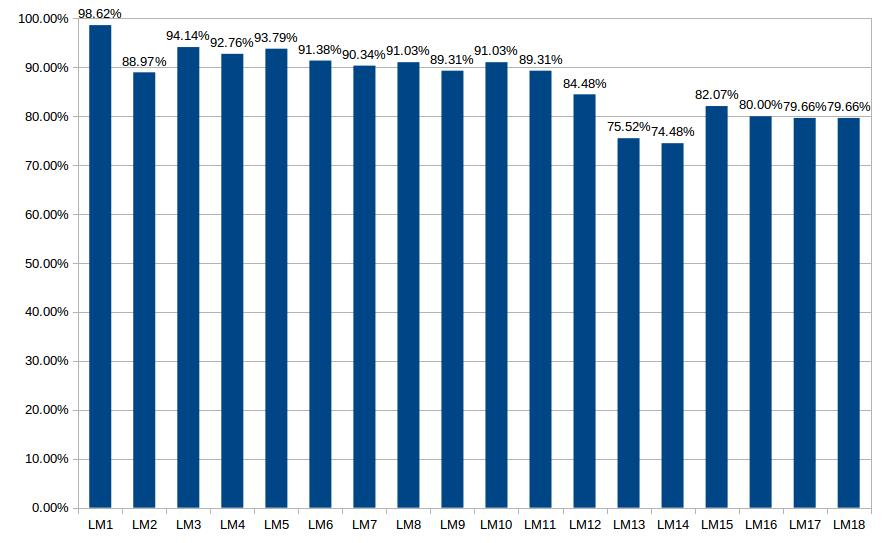
\includegraphics[width=0.5\textwidth]{./images/md_chartlms}
    \caption{The correct proportions on each landmark of right mandibles }
    \label{figmdresultlm}
\end{figure}~\\
\begin{figure}[htb]
    \centering
    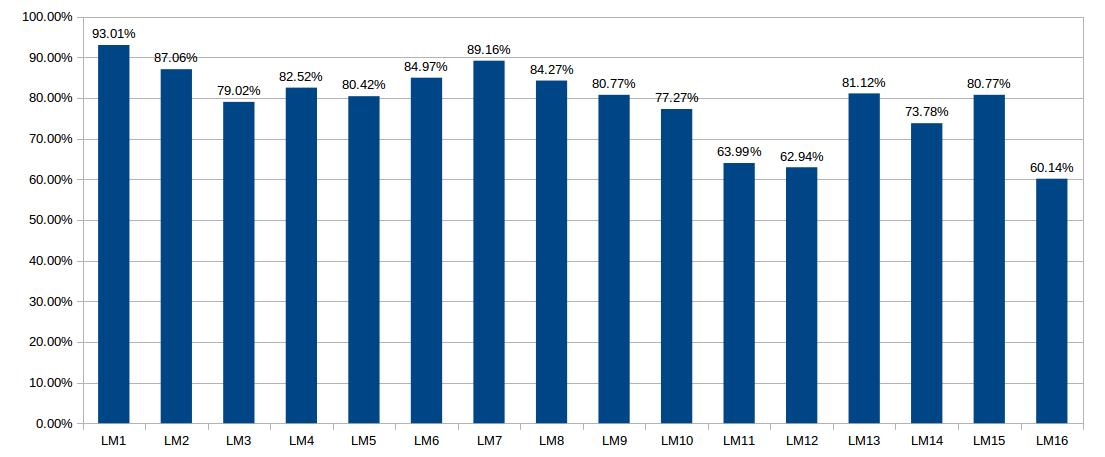
\includegraphics[width=0.5\textwidth]{./images/mg_chartlms}
    \caption{The correct proportions on each landmark of left mandibles }
    \label{figmgresultlm}
\end{figure}~\\
Figure \ref{figmdresultlm} and \ref{figmgresultlm} show the correct proportion on each landmark of mandible. The blue column is presented for the success rate. The orange column is expressed as the incorrect rate. With 18 landmarks of right mandible, the position of the first automatic landmarks is reasonably accurate with 98.62\%, the lowest proportion is 73,1\% for fourteenth landmark. The remaining landmarks are also indicated with a high proportion (with the accuracy proportion greater than 80\%). For left mandible, the highest and lowest success rate are 94,41\% for the first landmark and 58,04\% for the eleventh landmark. As we see, the images in left mandible are having more type of size than on the right mandible. This explains why the success rate on right mandible is higher than left mandible.\\

From two experiment ways, we can see that the method is success in
indicating all landmarks for each image; and the location of the
landmarks is considered near with the manual landmarks in some
aspect.\\

In a different side, when comparing with our previous study (see in
\cite{leestimating}). This method has more exactly about the position of
automatic landmarks as well as the advantages for the implementation
process. The memory to detecting the landmarks, along with the times
to execute the process are decreased dramatically.

\section{Conclusion}
Morphometric analysis is a powerful tool in biology in classification
the species. Automatic identification the characteristics biology of
the organism is a difficult problem. In the content of this paper, we
have begun to design a method to segment the beetle mandibles and to
indicate automatically landmarks which have been determined by
biologists. Each mandible is segmented by applying the Canny
algorithm. Using GHT and image registration to estimate the
landmarks. Finally, a descriptor distance will be applied to refine the
location of the estimated landmarks. The first version of this method
has been implemented. From now, the next stage of our method is to add
the features to have the position of landmarks more precisely, i.e diagnose on the scale of the image.


\bibliographystyle{plain}
\bibliography{references}

\end{document}

%-------------------------------------------------------------------------
% example of algorithm typesetting
% to allow this, uncomment line 
% \RequirePackage[noend]{myalgorithm}
% in the wscg.sty file
% and download that package from Gabriel Zachmann's page http://zach.in.tu-clausthal.de/latex/
%
%
%\begin{algorithm}
%\hrule
%  \centering
%\begin{algorithmic}
%    \STMT $d_{l,r} = f_B(P_1), f_B(P_n)$
%    \WHILE{ $|d_l| > \epsilon $ and $|d_r| > \epsilon $ and $l<r$}
%        \STMT $d_x = f_B(P_x)$
%        \IF{ $d_x < 0$ }
%            \STMT $l, r = x, r$
%        \ELSE
%            \STMT $l, r = l, x$
%        \ENDIF
%    \ENDWHILE
%\end{algorithmic}
%\hrule
%\caption{Example of some pseudo-code}
%\label{fg:code}
%\end{algorithm}

%-------------------------------------------------------------------------

\begin{thebibliography}{99}
\label{references}
\bibitem[1]{canny} Canny, John. "A computational approach to edge detection." IEEE Transactions on pattern analysis and machine intelligence 6 (1986): 679-698.
\bibitem[2]{Ballard} Ballard, Dana H. "Generalizing the Hough transform to detect arbitrary shapes." Pattern recognition 13.2 (1981): 111-122.
\bibitem[3]{Webster} Webster, M. A. R. K., and H. DAVID Sheets. "A practical introduction to landmark-based geometric morphometrics." Quantitative Methods in Paleobiology 16 (2010): 168-188.
\bibitem[4]{est} Le Van, L., et al. "Estimating landmarks on 2D images of beetle mandibles."
\bibitem[5]{pca} Shlens, Jonathon. "A tutorial on principal component analysis." arXiv preprint arXiv:1404.1100 (2014).
\bibitem[6]{sift} Lowe, David G. "Distinctive image features from scale-invariant keypoints." International journal of computer vision 60.2 (2004): 91-110.
\bibitem[7]{palaniswamy} Palaniswamy, Sasirekha, Neil A. Thacker, and Christian Peter Klingenberg. "Automatic identification of landmarks in digital images." IET Computer Vision 4.4 (2010): 247-260.
\end{thebibliography}

%{\bfseries
%Last page should be fully used by text, figures etc. Do not leave empty space, please. 

%Do not lock the PDF -- additional text and info will be inserted, i.e. ISSN/ISBN etc. 
%}

